% time values for run11, run14 and run15
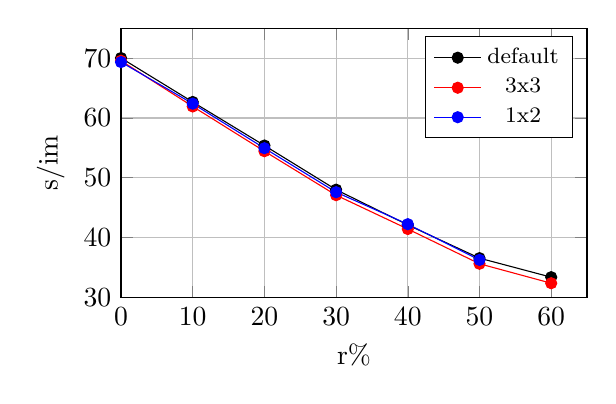
\begin{tikzpicture}
\begin{axis}[
    title={},
    height=5cm,
    width=7.5cm,
    xlabel={r\%},
    ylabel={s/im},
    xmin=0, xmax=65,
    ymin=30, ymax=75,
    xtick={0,10,20,30,40,50,60},
    ytick={30,40,50,60,70},
    legend pos=north east,
    xmajorgrids=true,
    ymajorgrids=true,
    legend style={font=\footnotesize}
]

\addplot[
    color=black,
    mark=*
    ]
    coordinates {
    (0,70.02)(10,62.67)(20,55.39)(30,48.01)(40,42.11)(50,36.56)(60,33.38)
    };
    
\addplot[
    color=red,
    mark=*
    ]
    coordinates {
    (0,69.56)(10,61.92)(20,54.44)(30,47.09)(40,41.43)(50,35.62)(60,32.37)
    };

\addplot[
    color=blue,
    mark=*
    ]
    coordinates {
    (0,69.34)(10,62.39)(20,54.94)(30,47.59)(40,42.24)(50,36.27)
    };
    
\legend{default, 3x3, 1x2}
    
\end{axis}
\end{tikzpicture}